\documentclass[1p]{elsarticle_modified}
%\bibliographystyle{elsarticle-num}

%\usepackage[colorlinks]{hyperref}
%\usepackage{abbrmath_seonhwa} %\Abb, \Ascr, \Acal ,\Abf, \Afrak
\usepackage{amsfonts}
\usepackage{amssymb}
\usepackage{amsmath}
\usepackage{amsthm}
\usepackage{scalefnt}
\usepackage{amsbsy}
\usepackage{kotex}
\usepackage{caption}
\usepackage{subfig}
\usepackage{color}
\usepackage{graphicx}
\usepackage{xcolor} %% white, black, red, green, blue, cyan, magenta, yellow
\usepackage{float}
\usepackage{setspace}
\usepackage{hyperref}

\usepackage{tikz}
\usetikzlibrary{arrows}

\usepackage{multirow}
\usepackage{array} % fixed length table
\usepackage{hhline}

%%%%%%%%%%%%%%%%%%%%%
\makeatletter
\renewcommand*\env@matrix[1][\arraystretch]{%
	\edef\arraystretch{#1}%
	\hskip -\arraycolsep
	\let\@ifnextchar\new@ifnextchar
	\array{*\c@MaxMatrixCols c}}
\makeatother %https://tex.stackexchange.com/questions/14071/how-can-i-increase-the-line-spacing-in-a-matrix
%%%%%%%%%%%%%%%

\usepackage[normalem]{ulem}

\newcommand{\msout}[1]{\ifmmode\text{\sout{\ensuremath{#1}}}\else\sout{#1}\fi}
%SOURCE: \msout is \stkout macro in https://tex.stackexchange.com/questions/20609/strikeout-in-math-mode

\newcommand{\cancel}[1]{
	\ifmmode
	{\color{red}\msout{#1}}
	\else
	{\color{red}\sout{#1}}
	\fi
}

\newcommand{\add}[1]{
	{\color{blue}\uwave{#1}}
}

\newcommand{\replace}[2]{
	\ifmmode
	{\color{red}\msout{#1}}{\color{blue}\uwave{#2}}
	\else
	{\color{red}\sout{#1}}{\color{blue}\uwave{#2}}
	\fi
}

\newcommand{\Sol}{\mathcal{S}} %segment
\newcommand{\D}{D} %diagram
\newcommand{\A}{\mathcal{A}} %arc


%%%%%%%%%%%%%%%%%%%%%%%%%%%%%5 test

\def\sl{\operatorname{\textup{SL}}(2,\Cbb)}
\def\psl{\operatorname{\textup{PSL}}(2,\Cbb)}
\def\quan{\mkern 1mu \triangleright \mkern 1mu}

\theoremstyle{definition}
\newtheorem{thm}{Theorem}[section]
\newtheorem{prop}[thm]{Proposition}
\newtheorem{lem}[thm]{Lemma}
\newtheorem{ques}[thm]{Question}
\newtheorem{cor}[thm]{Corollary}
\newtheorem{defn}[thm]{Definition}
\newtheorem{exam}[thm]{Example}
\newtheorem{rmk}[thm]{Remark}
\newtheorem{alg}[thm]{Algorithm}

\newcommand{\I}{\sqrt{-1}}
\begin{document}

%\begin{frontmatter}
%
%\title{Boundary parabolic representations of knots up to 8 crossings}
%
%%% Group authors per affiliation:
%\author{Yunhi Cho} 
%\address{Department of Mathematics, University of Seoul, Seoul, Korea}
%\ead{yhcho@uos.ac.kr}
%
%
%\author{Seonhwa Kim} %\fnref{s_kim}}
%\address{Center for Geometry and Physics, Institute for Basic Science, Pohang, 37673, Korea}
%\ead{ryeona17@ibs.re.kr}
%
%\author{Hyuk Kim}
%\address{Department of Mathematical Sciences, Seoul National University, Seoul 08826, Korea}
%\ead{hyukkim@snu.ac.kr}
%
%\author{Seokbeom Yoon}
%\address{Department of Mathematical Sciences, Seoul National University, Seoul, 08826,  Korea}
%\ead{sbyoon15@snu.ac.kr}
%
%\begin{abstract}
%We find all boundary parabolic representation of knots up to 8 crossings.
%
%\end{abstract}
%\begin{keyword}
%    \MSC[2010] 57M25 
%\end{keyword}
%
%\end{frontmatter}

%\linenumbers
%\tableofcontents
%
\newcommand\colored[1]{\textcolor{white}{\rule[-0.35ex]{0.8em}{1.4ex}}\kern-0.8em\color{red} #1}%
%\newcommand\colored[1]{\textcolor{white}{ #1}\kern-2.17ex	\textcolor{white}{ #1}\kern-1.81ex	\textcolor{white}{ #1}\kern-2.15ex\color{red}#1	}

{\Large $\underline{12a_{0797}~(K12a_{0797})}$}

\setlength{\tabcolsep}{10pt}
\renewcommand{\arraystretch}{1.6}
\vspace{1cm}\begin{tabular}{m{100pt}>{\centering\arraybackslash}m{274pt}}
\multirow{5}{120pt}{
	\centering
	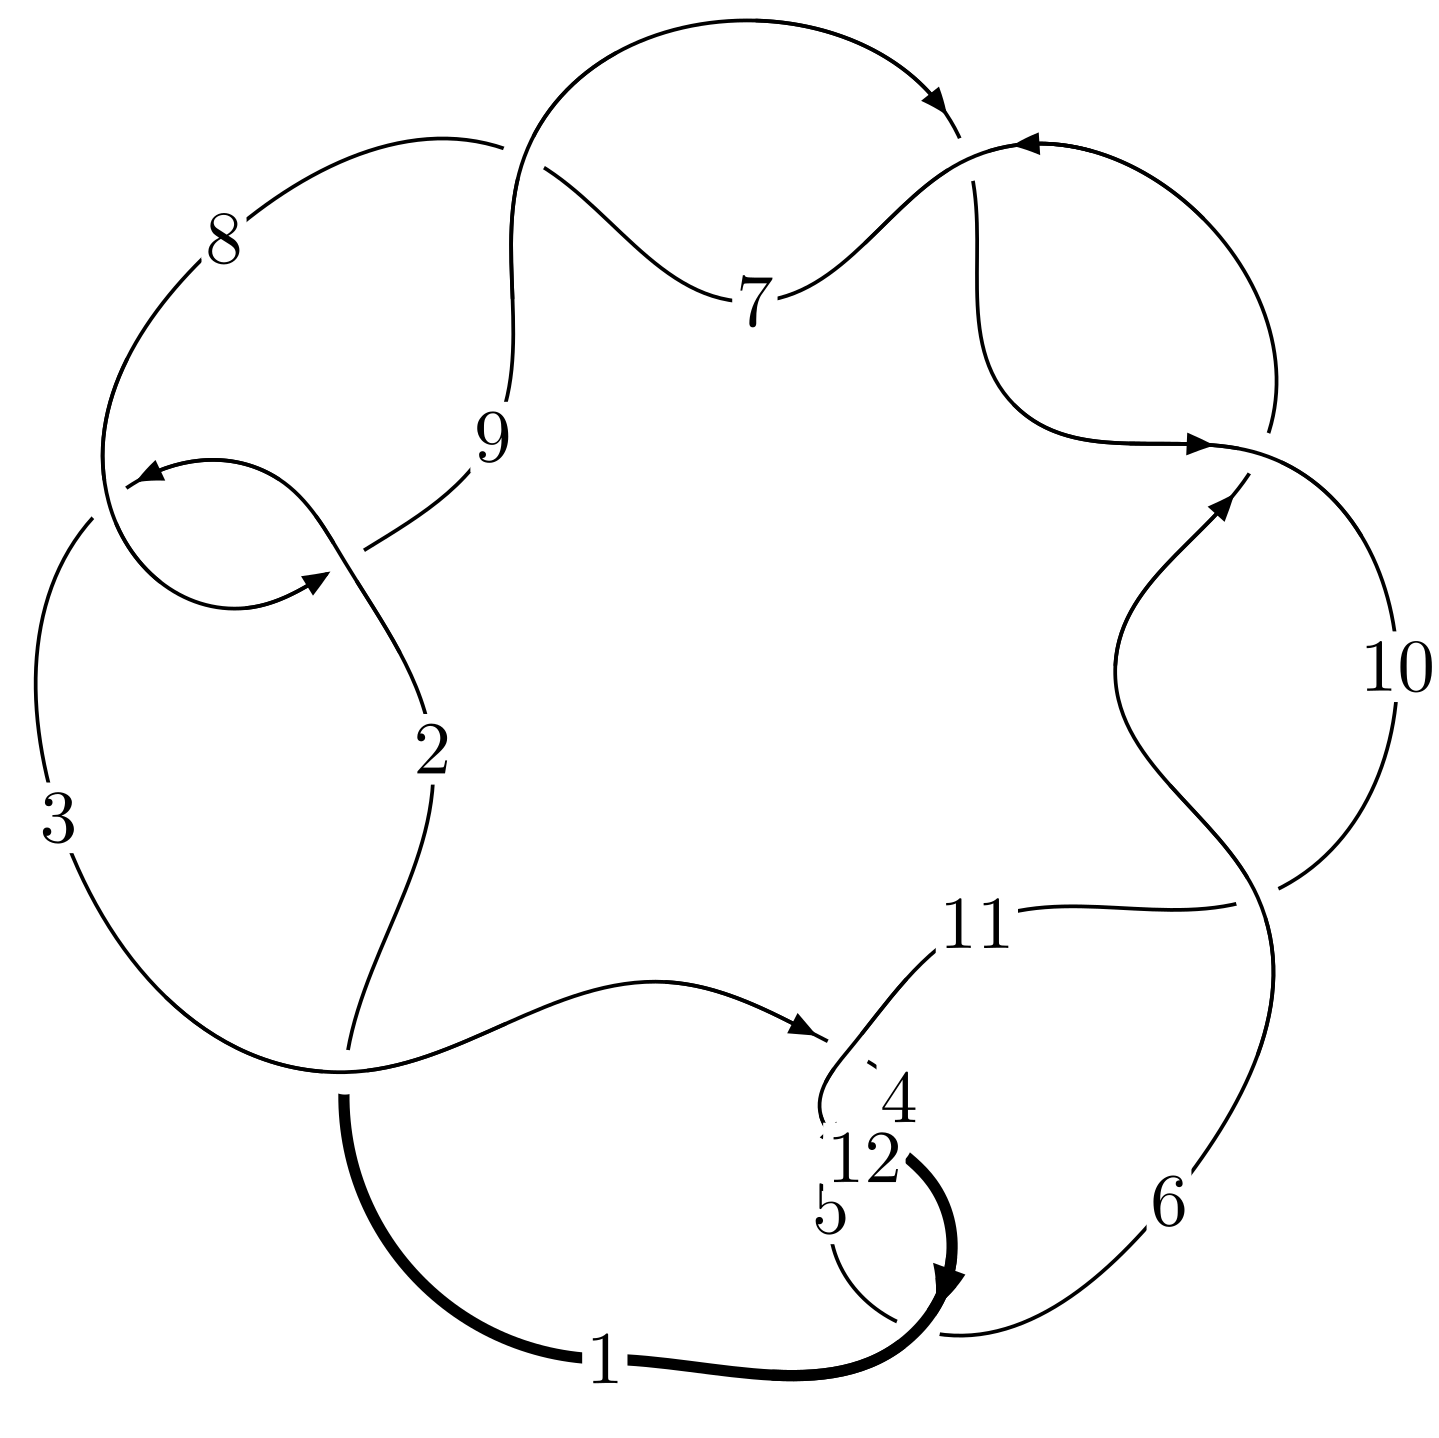
\includegraphics[width=112pt]{../../../GIT/diagram.site/Diagrams/png/1598_12a_0797.png}\\
\ \ \ A knot diagram\footnotemark}&
\allowdisplaybreaks
\textbf{Linearized knot diagam} \\
\cline{2-2}
 &
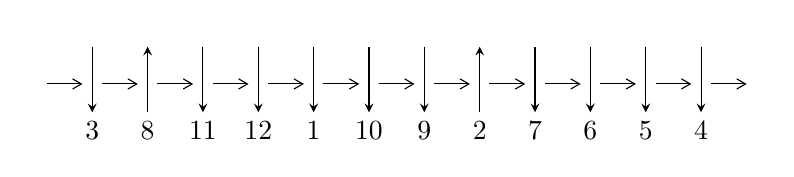
\begin{tikzpicture}[x=20pt, y=17pt]
	% nodes
	\node (C0) at (0, 0) {};
	\node (C1) at (1, 0) {};
	\node (C1U) at (1, +1) {};
	\node (C1D) at (1, -1) {3};

	\node (C2) at (2, 0) {};
	\node (C2U) at (2, +1) {};
	\node (C2D) at (2, -1) {8};

	\node (C3) at (3, 0) {};
	\node (C3U) at (3, +1) {};
	\node (C3D) at (3, -1) {11};

	\node (C4) at (4, 0) {};
	\node (C4U) at (4, +1) {};
	\node (C4D) at (4, -1) {12};

	\node (C5) at (5, 0) {};
	\node (C5U) at (5, +1) {};
	\node (C5D) at (5, -1) {1};

	\node (C6) at (6, 0) {};
	\node (C6U) at (6, +1) {};
	\node (C6D) at (6, -1) {10};

	\node (C7) at (7, 0) {};
	\node (C7U) at (7, +1) {};
	\node (C7D) at (7, -1) {9};

	\node (C8) at (8, 0) {};
	\node (C8U) at (8, +1) {};
	\node (C8D) at (8, -1) {2};

	\node (C9) at (9, 0) {};
	\node (C9U) at (9, +1) {};
	\node (C9D) at (9, -1) {7};

	\node (C10) at (10, 0) {};
	\node (C10U) at (10, +1) {};
	\node (C10D) at (10, -1) {6};

	\node (C11) at (11, 0) {};
	\node (C11U) at (11, +1) {};
	\node (C11D) at (11, -1) {5};

	\node (C12) at (12, 0) {};
	\node (C12U) at (12, +1) {};
	\node (C12D) at (12, -1) {4};
	\node (C13) at (13, 0) {};

	% arrows
	\draw[->,>={angle 60}]
	(C0) edge (C1) (C1) edge (C2) (C2) edge (C3) (C3) edge (C4) (C4) edge (C5) (C5) edge (C6) (C6) edge (C7) (C7) edge (C8) (C8) edge (C9) (C9) edge (C10) (C10) edge (C11) (C11) edge (C12) (C12) edge (C13) ;	\draw[->,>=stealth]
	(C1U) edge (C1D) (C2D) edge (C2U) (C3U) edge (C3D) (C4U) edge (C4D) (C5U) edge (C5D) (C6U) edge (C6D) (C7U) edge (C7D) (C8D) edge (C8U) (C9U) edge (C9D) (C10U) edge (C10D) (C11U) edge (C11D) (C12U) edge (C12D) ;
	\end{tikzpicture} \\
\hhline{~~} \\& 
\textbf{Solving Sequence} \\ \cline{2-2} 
 &
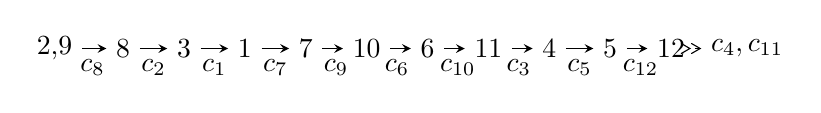
\begin{tikzpicture}[x=22pt, y=7pt]
	% node
	\node (A0) at (-1/8, 0) {2,9};
	\node (A1) at (1, 0) {8};
	\node (A2) at (2, 0) {3};
	\node (A3) at (3, 0) {1};
	\node (A4) at (4, 0) {7};
	\node (A5) at (5, 0) {10};
	\node (A6) at (6, 0) {6};
	\node (A7) at (7, 0) {11};
	\node (A8) at (8, 0) {4};
	\node (A9) at (9, 0) {5};
	\node (A10) at (10, 0) {12};
	\node (C1) at (1/2, -1) {$c_{8}$};
	\node (C2) at (3/2, -1) {$c_{2}$};
	\node (C3) at (5/2, -1) {$c_{1}$};
	\node (C4) at (7/2, -1) {$c_{7}$};
	\node (C5) at (9/2, -1) {$c_{9}$};
	\node (C6) at (11/2, -1) {$c_{6}$};
	\node (C7) at (13/2, -1) {$c_{10}$};
	\node (C8) at (15/2, -1) {$c_{3}$};
	\node (C9) at (17/2, -1) {$c_{5}$};
	\node (C10) at (19/2, -1) {$c_{12}$};
	\node (A11) at (45/4, 0) {$c_{4},c_{11}$};

	% edge
	\draw[->,>=stealth]	
	(A0) edge (A1) (A1) edge (A2) (A2) edge (A3) (A3) edge (A4) (A4) edge (A5) (A5) edge (A6) (A6) edge (A7) (A7) edge (A8) (A8) edge (A9) (A9) edge (A10) ;
	\draw[->>,>={angle 60}]	
	(A10) edge (A11);
\end{tikzpicture} \\ 

\end{tabular} \\

\footnotetext{
The image of knot diagram is generated by the software ``\textbf{Draw programme}" developed by Andrew Bartholomew(\url{http://www.layer8.co.uk/maths/draw/index.htm\#Running-draw}), where we modified some parts for our purpose(\url{https://github.com/CATsTAILs/LinksPainter}).
}\phantom \\ \newline 
\centering \textbf{Ideals for irreducible components\footnotemark of $X_{\text{par}}$} 
 
\begin{align*}
I^u_{1}&=\langle 
u^{41}+u^{40}+\cdots- u-1\rangle \\
\\
\end{align*}
\raggedright * 1 irreducible components of $\dim_{\mathbb{C}}=0$, with total 41 representations.\\
\footnotetext{All coefficients of polynomials are rational numbers. But the coefficients are sometimes approximated in decimal forms when there is not enough margin.}
\newpage
\renewcommand{\arraystretch}{1}
\centering \section*{I. $I^u_{1}= \langle u^{41}+u^{40}+\cdots- u-1 \rangle$}
\flushleft \textbf{(i) Arc colorings}\\
\begin{tabular}{m{7pt} m{180pt} m{7pt} m{180pt} }
\flushright $a_{2}=$&$\begin{pmatrix}0\\u\end{pmatrix}$ \\
\flushright $a_{9}=$&$\begin{pmatrix}1\\0\end{pmatrix}$ \\
\flushright $a_{8}=$&$\begin{pmatrix}1\\u^2\end{pmatrix}$ \\
\flushright $a_{3}=$&$\begin{pmatrix}u\\u^3+u\end{pmatrix}$ \\
\flushright $a_{1}=$&$\begin{pmatrix}u^3\\u^5+u^3+u\end{pmatrix}$ \\
\flushright $a_{7}=$&$\begin{pmatrix}u^2+1\\u^2\end{pmatrix}$ \\
\flushright $a_{10}=$&$\begin{pmatrix}u^4+u^2+1\\u^4\end{pmatrix}$ \\
\flushright $a_{6}=$&$\begin{pmatrix}u^6+u^4+2 u^2+1\\u^6+u^2\end{pmatrix}$ \\
\flushright $a_{11}=$&$\begin{pmatrix}u^8+u^6+3 u^4+2 u^2+1\\u^8+2 u^4\end{pmatrix}$ \\
\flushright $a_{4}=$&$\begin{pmatrix}- u^{19}-2 u^{17}-8 u^{15}-12 u^{13}-21 u^{11}-22 u^9-20 u^7-12 u^5-5 u^3\\- u^{19}- u^{17}-6 u^{15}-5 u^{13}-11 u^{11}-7 u^9-6 u^7-2 u^5+u^3+u\end{pmatrix}$ \\
\flushright $a_{5}=$&$\begin{pmatrix}- u^{14}- u^{12}-4 u^{10}-3 u^8-2 u^6+2 u^2+1\\- u^{16}-2 u^{14}-6 u^{12}-8 u^{10}-10 u^8-6 u^6-4 u^4\end{pmatrix}$ \\
\flushright $a_{12}=$&$\begin{pmatrix}u^{38}+3 u^{36}+\cdots+2 u^2+1\\u^{40}+4 u^{38}+\cdots+25 u^8+2 u^4\end{pmatrix}$\\&\end{tabular}
\flushleft \textbf{(ii) Obstruction class $= -1$}\\~\\
\flushleft \textbf{(iii) Cusp Shapes $= -4 u^{40}-12 u^{38}+4 u^{37}-72 u^{36}+12 u^{35}-172 u^{34}+68 u^{33}-532 u^{32}+156 u^{31}-1020 u^{30}+456 u^{29}-2104 u^{28}+808 u^{27}-3232 u^{26}+1556 u^{25}-4840 u^{24}+2116 u^{23}-5884 u^{22}+2876 u^{21}-6544 u^{20}+2924 u^{19}-6116 u^{18}+2796 u^{17}-4940 u^{16}+1988 u^{15}-3316 u^{14}+1224 u^{13}-1768 u^{12}+472 u^{11}-688 u^{10}+92 u^9-148 u^8-68 u^7+24 u^6-44 u^5+24 u^4-24 u^3-4 u^2+8 u-6$}\\~\\
\newpage\renewcommand{\arraystretch}{1}
\flushleft \textbf{(iv) u-Polynomials at the component}\newline \\
\begin{tabular}{m{50pt}|m{274pt}}
Crossings & \hspace{64pt}u-Polynomials at each crossing \\
\hline $$\begin{aligned}c_{1},c_{6},c_{7}\\c_{9},c_{10}\end{aligned}$$&$\begin{aligned}
&u^{41}+7 u^{40}+\cdots-3 u-1
\end{aligned}$\\
\hline $$\begin{aligned}c_{2},c_{8}\end{aligned}$$&$\begin{aligned}
&u^{41}- u^{40}+\cdots- u+1
\end{aligned}$\\
\hline $$\begin{aligned}c_{3},c_{5}\end{aligned}$$&$\begin{aligned}
&u^{41}+u^{40}+\cdots+7 u+1
\end{aligned}$\\
\hline $$\begin{aligned}c_{4},c_{11},c_{12}\end{aligned}$$&$\begin{aligned}
&u^{41}- u^{40}+\cdots+3 u+1
\end{aligned}$\\
\hline
\end{tabular}\\~\\
\newpage\renewcommand{\arraystretch}{1}
\flushleft \textbf{(v) Riley Polynomials at the component}\newline \\
\begin{tabular}{m{50pt}|m{274pt}}
Crossings & \hspace{64pt}Riley Polynomials at each crossing \\
\hline $$\begin{aligned}c_{1},c_{6},c_{7}\\c_{9},c_{10}\end{aligned}$$&$\begin{aligned}
&y^{41}+55 y^{40}+\cdots+21 y-1
\end{aligned}$\\
\hline $$\begin{aligned}c_{2},c_{8}\end{aligned}$$&$\begin{aligned}
&y^{41}+7 y^{40}+\cdots-3 y-1
\end{aligned}$\\
\hline $$\begin{aligned}c_{3},c_{5}\end{aligned}$$&$\begin{aligned}
&y^{41}-17 y^{40}+\cdots-3 y-1
\end{aligned}$\\
\hline $$\begin{aligned}c_{4},c_{11},c_{12}\end{aligned}$$&$\begin{aligned}
&y^{41}+35 y^{40}+\cdots-3 y-1
\end{aligned}$\\
\hline
\end{tabular}\\~\\
\newpage\flushleft \textbf{(vi) Complex Volumes and Cusp Shapes}
$$\begin{array}{c|c|c}  
\text{Solutions to }I^u_{1}& \I (\text{vol} + \sqrt{-1}CS) & \text{Cusp shape}\\
 \hline 
\begin{aligned}
u &= \phantom{-}0.746721 + 0.668302 I\end{aligned}
 & \phantom{-}6.12347 - 4.43186 I & -0.64976 + 2.52749 I \\ \hline\begin{aligned}
u &= \phantom{-}0.746721 - 0.668302 I\end{aligned}
 & \phantom{-}6.12347 + 4.43186 I & -0.64976 - 2.52749 I \\ \hline\begin{aligned}
u &= \phantom{-}0.640826 + 0.762779 I\end{aligned}
 & \phantom{-}3.41343 + 2.37839 I & -1.91604 - 4.49876 I \\ \hline\begin{aligned}
u &= \phantom{-}0.640826 - 0.762779 I\end{aligned}
 & \phantom{-}3.41343 - 2.37839 I & -1.91604 + 4.49876 I \\ \hline\begin{aligned}
u &= \phantom{-}0.577712 + 0.822944 I\end{aligned}
 & \phantom{-}3.32469 + 2.15500 I & -4.15170 - 3.81656 I \\ \hline\begin{aligned}
u &= \phantom{-}0.577712 - 0.822944 I\end{aligned}
 & \phantom{-}3.32469 - 2.15500 I & -4.15170 + 3.81656 I \\ \hline\begin{aligned}
u &= -0.699230 + 0.665301 I\end{aligned}
 & \phantom{-}1.31088 + 0.84318 I & -5.61398 - 1.15748 I \\ \hline\begin{aligned}
u &= -0.699230 - 0.665301 I\end{aligned}
 & \phantom{-}1.31088 - 0.84318 I & -5.61398 + 1.15748 I \\ \hline\begin{aligned}
u &= -0.624667 + 0.879172 I\end{aligned}
 & \phantom{-}0.61729 - 5.77850 I & -7.67117 + 7.41312 I \\ \hline\begin{aligned}
u &= -0.624667 - 0.879172 I\end{aligned}
 & \phantom{-}0.61729 + 5.77850 I & -7.67117 - 7.41312 I \\ \hline\begin{aligned}
u &= -0.729895 + 0.807771 I\end{aligned}
 & \phantom{-}9.55876 - 2.69232 I & \phantom{-}1.62765 + 3.28476 I \\ \hline\begin{aligned}
u &= -0.729895 - 0.807771 I\end{aligned}
 & \phantom{-}9.55876 + 2.69232 I & \phantom{-}1.62765 - 3.28476 I \\ \hline\begin{aligned}
u &= -0.261594 + 0.866448 I\end{aligned}
 & \phantom{-}0.30761 - 5.87325 I & -8.98780 + 8.12941 I \\ \hline\begin{aligned}
u &= -0.261594 - 0.866448 I\end{aligned}
 & \phantom{-}0.30761 + 5.87325 I & -8.98780 - 8.12941 I \\ \hline\begin{aligned}
u &= \phantom{-}0.646192 + 0.901469 I\end{aligned}
 & \phantom{-}5.35322 + 9.58701 I & -2.83138 - 8.65051 I \\ \hline\begin{aligned}
u &= \phantom{-}0.646192 - 0.901469 I\end{aligned}
 & \phantom{-}5.35322 - 9.58701 I & -2.83138 + 8.65051 I \\ \hline\begin{aligned}
u &= \phantom{-}0.211383 + 0.848155 I\end{aligned}
 & -3.89636 + 2.17908 I & -14.9383 - 5.2468 I \\ \hline\begin{aligned}
u &= \phantom{-}0.211383 - 0.848155 I\end{aligned}
 & -3.89636 - 2.17908 I & -14.9383 + 5.2468 I \\ \hline\begin{aligned}
u &= -0.143224 + 0.847989 I\end{aligned}
 & -0.30668 + 1.42021 I & -11.22317 + 0.51661 I \\ \hline\begin{aligned}
u &= -0.143224 - 0.847989 I\end{aligned}
 & -0.30668 - 1.42021 I & -11.22317 - 0.51661 I \\ \hline\begin{aligned}
u &= \phantom{-}0.536289 + 0.522200 I\end{aligned}
 & \phantom{-}3.94243 + 1.95655 I & -0.40351 - 3.68221 I \\ \hline\begin{aligned}
u &= \phantom{-}0.536289 - 0.522200 I\end{aligned}
 & \phantom{-}3.94243 - 1.95655 I & -0.40351 + 3.68221 I \\ \hline\begin{aligned}
u &= -0.918409 + 0.933266 I\end{aligned}
 & \phantom{-}12.96880 - 3.08508 I & -2.25641 + 3.40948 I \\ \hline\begin{aligned}
u &= -0.918409 - 0.933266 I\end{aligned}
 & \phantom{-}12.96880 + 3.08508 I & -2.25641 - 3.40948 I \\ \hline\begin{aligned}
u &= \phantom{-}0.928532 + 0.923939 I\end{aligned}
 & \phantom{-}10.84470 - 1.03628 I & -5.06255 + 1.18461 I \\ \hline\begin{aligned}
u &= \phantom{-}0.928532 - 0.923939 I\end{aligned}
 & \phantom{-}10.84470 + 1.03628 I & -5.06255 - 1.18461 I \\ \hline\begin{aligned}
u &= -0.909755 + 0.948945 I\end{aligned}
 & \phantom{-}12.91700 - 3.64558 I & -2.38906 + 1.25453 I \\ \hline\begin{aligned}
u &= -0.909755 - 0.948945 I\end{aligned}
 & \phantom{-}12.91700 + 3.64558 I & -2.38906 - 1.25453 I \\ \hline\begin{aligned}
u &= -0.936924 + 0.922936 I\end{aligned}
 & \phantom{-}15.9484 + 4.9714 I & -0.68196 - 2.33270 I \\ \hline\begin{aligned}
u &= -0.936924 - 0.922936 I\end{aligned}
 & \phantom{-}15.9484 - 4.9714 I & -0.68196 + 2.33270 I\\
 \hline 
 \end{array}$$\newpage$$\begin{array}{c|c|c}  
\text{Solutions to }I^u_{1}& \I (\text{vol} + \sqrt{-1}CS) & \text{Cusp shape}\\
 \hline 
\begin{aligned}
u &= \phantom{-}0.908129 + 0.961589 I\end{aligned}
 & \phantom{-}10.72100 + 7.79340 I & -5.31261 - 5.70338 I \\ \hline\begin{aligned}
u &= \phantom{-}0.908129 - 0.961589 I\end{aligned}
 & \phantom{-}10.72100 - 7.79340 I & -5.31261 + 5.70338 I \\ \hline\begin{aligned}
u &= \phantom{-}0.930424 + 0.949937 I\end{aligned}
 & -19.2344 + 3.4189 I & \phantom{-}1.88979 - 2.27252 I \\ \hline\begin{aligned}
u &= \phantom{-}0.930424 - 0.949937 I\end{aligned}
 & -19.2344 - 3.4189 I & \phantom{-}1.88979 + 2.27252 I \\ \hline\begin{aligned}
u &= -0.911356 + 0.968477 I\end{aligned}
 & \phantom{-}15.7979 - 11.7662 I & -0.97634 + 6.84571 I \\ \hline\begin{aligned}
u &= -0.911356 - 0.968477 I\end{aligned}
 & \phantom{-}15.7979 + 11.7662 I & -0.97634 - 6.84571 I \\ \hline\begin{aligned}
u &= -0.193562 + 0.561475 I\end{aligned}
 & -0.310431 - 0.802598 I & -7.57849 + 8.41194 I \\ \hline\begin{aligned}
u &= -0.193562 - 0.561475 I\end{aligned}
 & -0.310431 + 0.802598 I & -7.57849 - 8.41194 I \\ \hline\begin{aligned}
u &= -0.534709 + 0.122960 I\end{aligned}
 & \phantom{-}2.61523 + 3.18305 I & -0.67808 - 2.90815 I \\ \hline\begin{aligned}
u &= -0.534709 - 0.122960 I\end{aligned}
 & \phantom{-}2.61523 - 3.18305 I & -0.67808 + 2.90815 I \\ \hline\begin{aligned}
u &= \phantom{-}0.474234\phantom{ +0.000000I}\end{aligned}
 & -1.44617\phantom{ +0.000000I} & -6.39030\phantom{ +0.000000I}\\
 \hline 
 \end{array}$$\newpage
\newpage\renewcommand{\arraystretch}{1}
\centering \section*{ II. u-Polynomials}
\begin{tabular}{m{50pt}|m{274pt}}
Crossings & \hspace{64pt}u-Polynomials at each crossing \\
\hline $$\begin{aligned}c_{1},c_{6},c_{7}\\c_{9},c_{10}\end{aligned}$$&$\begin{aligned}
&u^{41}+7 u^{40}+\cdots-3 u-1
\end{aligned}$\\
\hline $$\begin{aligned}c_{2},c_{8}\end{aligned}$$&$\begin{aligned}
&u^{41}- u^{40}+\cdots- u+1
\end{aligned}$\\
\hline $$\begin{aligned}c_{3},c_{5}\end{aligned}$$&$\begin{aligned}
&u^{41}+u^{40}+\cdots+7 u+1
\end{aligned}$\\
\hline $$\begin{aligned}c_{4},c_{11},c_{12}\end{aligned}$$&$\begin{aligned}
&u^{41}- u^{40}+\cdots+3 u+1
\end{aligned}$\\
\hline
\end{tabular}\newpage\renewcommand{\arraystretch}{1}
\centering \section*{ III. Riley Polynomials}
\begin{tabular}{m{50pt}|m{274pt}}
Crossings & \hspace{64pt}Riley Polynomials at each crossing \\
\hline $$\begin{aligned}c_{1},c_{6},c_{7}\\c_{9},c_{10}\end{aligned}$$&$\begin{aligned}
&y^{41}+55 y^{40}+\cdots+21 y-1
\end{aligned}$\\
\hline $$\begin{aligned}c_{2},c_{8}\end{aligned}$$&$\begin{aligned}
&y^{41}+7 y^{40}+\cdots-3 y-1
\end{aligned}$\\
\hline $$\begin{aligned}c_{3},c_{5}\end{aligned}$$&$\begin{aligned}
&y^{41}-17 y^{40}+\cdots-3 y-1
\end{aligned}$\\
\hline $$\begin{aligned}c_{4},c_{11},c_{12}\end{aligned}$$&$\begin{aligned}
&y^{41}+35 y^{40}+\cdots-3 y-1
\end{aligned}$\\
\hline
\end{tabular}
\vskip 2pc
\end{document}